\chapter{Operator}

参考\figurename\ref{fig:1-arch}，前面的章节主要介绍存储引擎，本章和下一章介绍执行引擎。SQL语句大体按照如下过程执行：将SQL语句翻译为关系表达式，然后经过逻辑优化阶段，对关系表达式做等价变换。物理优化阶段，根据数据库实例的统计特征选择合适的关系算子实现算法，最后得到执行计划。

\begin{figure}[H]
    \centering
    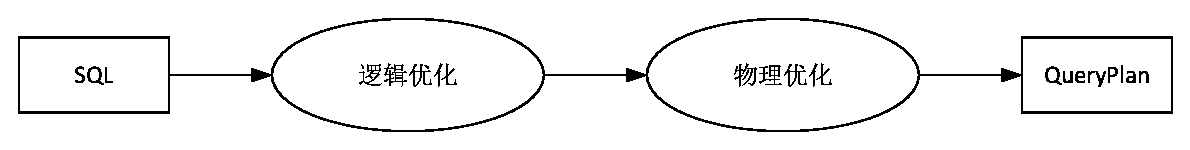
\includegraphics[width=\linewidth]{handout/img/5-plan.eps}
    \caption{SQL语句执行过程}\label{fig:5-plan}
\end{figure}

本章主要介绍如何实现表的交、并、连接、乘积等操作，这些操作会被使用在下一章的SQL解析中。一个关系模型算子可能有多种实现方式，需要关注是算子实现的性能、内存开销，同时本章还将讨论如何将算子连接以实现算子表达式。

\section{关系操作}

在讨论关系模型的算子具体实现之前，本节先回顾关系模型及其主要操作，介绍bag模型，最后讨论算法评估指标与参数。

\subsection{关系代数}

关系数据库的数据模型是\emph{关系}，数据模型是一个用于描述数据组织的抽象概念，它并非是数据库中具体实现的数据结构，而是是一个高层次的逻辑概念。一般将数据库中实现的的数据结构称为\emph{物理模型}，而称数据模型为\emph{概念模型}。数据模型的准确抽象是一类数据库成熟的标志。

在数据模型之上，数据库会定义各种操作。操作即函数，函数的参数是数据模型，后文将操作又称为算子。算子组合为算子表达式，以SQL为例，查询语句最终会被映射成一个算子表达式的实现。最后，应用采用数据模型来描述，仍然存在一些特性未能完全反应设计者的需求，比如数据完整性等，数据库需要提供一些特定的约束手段，如触发器等。

简单地说，关系就是一张二维的表，横向是行，纵向是列。横向称为tuple或者记录，纵向称为属性。每个属性都有名字，关系的属性构成一个集合，称为schema。通常一个关系的schema是固定的，属性集合是不变的，但schema与属性的排列顺序无关。逻辑上，关系的tuple如何排列也是无关的。

所谓\emph{关系代数}是指关系的操作结果仍然是关系，这样关系及其运算就构成了一个封闭的代数系统。关系的操作符有：
\begin{itemize}
    \item 单目操作，即操作符后只跟一个关系：
          \begin{enumerate}
              \item $\tau(R)$，对关系$R$做排序操作
              \item $\sigma_C(R)$，对关系$R$做选择操作，选择条件是$C$
              \item $\pi_E(R)$，对关系$R$做投影操作，投影的属性列表是$E$
              \item $\gamma_C(R)$，对关系$R$做分组，分组后的tuple做聚合操作$C$
              \item $\delta(R)$，对关系$R$去重，适用于后文的bag模型
          \end{enumerate}

    \item 双目操作，即操作符后跟两个关系：
          \begin{enumerate}
              \item $R \cap S$，关系$R$和$S$做交操作
              \item $R \cup S$，关系$R$和$S$做并操作
              \item $R - S$，关系$R$和$S$做差操作
              \item $R \times S$，关系$R$和$S$做笛卡尔积操作
              \item $R \bowtie S$，关系$R$和$S$做自然连接操作
              \item $R \bowtie_C S$，关系$R$和$S$做$\theta$连接操作，条件是$C$
          \end{enumerate}
\end{itemize}

\begin{exercise}
    单目、双目，有没有三目操作？
\end{exercise}

\subsection{bag模型}

虽然关系数据库的数据模型是关系，是tuple的集合，逻辑上不应该存在相同的tuple，但商用数据库通常采用bag数据模型，即允许关系中多次出现相同的tuple。原因是bag模型的算法实现更简单方便。例如，两个关系做并操作，$R \cup S$，如果是bag模型，简单地将所有tuple收集起来即可。

基于bag模型的关系操作，比关系模型的操作多一个$\delta$去重算子，除此外两者的算子语义有所不同，后文特别用下标$_B$表示bag模型操作。

\subsubsection*{投影$\pi_B$}

设$R$是bag模型的关系，对$R$做属性列表$E$的投影$\pi_E(R)$。结果可能出现多个相同的tuple，但结果的tuple数目与$R$相同。

\subsubsection*{选择$\sigma_B$}

设$R$是bag模型的关系，对$R$做条件为$C$的选择$\sigma_C(R)$，结果可能出现多个相同的tuple。

\subsubsection*{并$\cup_B$}

设$R$和$S$是两个bag模型的关系，一个tuple在$R$中出现$n$次，在$S$中出现$m$次，则$R \cup_B S$中，该tuple出现$n+m$次。

\subsubsection*{交$\cap_B$}

设$R$和$S$是两个bag模型的关系，一个tuple在$R$中出现$n$次，在$S$中出现$m$次，则$R \cap_B S$中，该tuple出现$min(n,m)$次。

\subsubsection*{差$-_B$}

设$R$和$S$是两个bag模型的关系，一个tuple在$R$中出现$n$次，在$S$中出现$m$次，则$R -_B S$中，该tuple出现$max(0,n-m)$次，当$n \le m$时出现$0$次，当$n \ge m$时出现$n-m$次。

\subsubsection*{积$\times_B$}

设$R$和$S$是两个bag模型的关系，则$R \times_B S$中，结果可能出现多个相同的tuple，数目为为$n \times m$。

\subsubsection*{连接$\bowtie_B$}

设$R$和$S$是两个bag模型的关系，则$R \bowtie_B S$中，结果可能出现多个相同的tuple。

\begin{figure}[H]
    \centering
    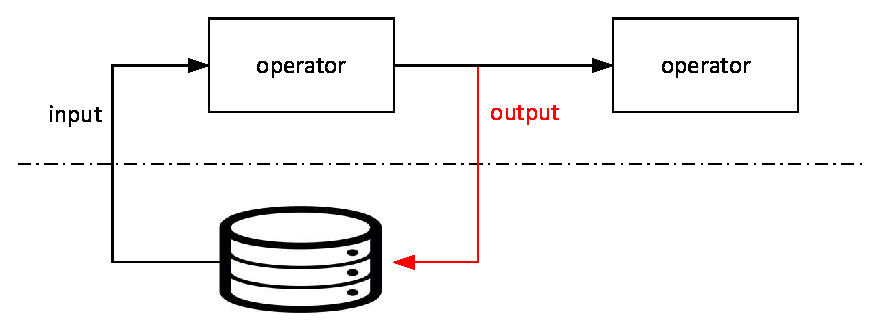
\includegraphics[width=0.8\linewidth]{handout/img/5-io.eps}
    \caption{operator连接与评估指标}\label{fig:5-io}
\end{figure}

\subsection{评估指标}

本章在比较各种操作的性能时，仍然使用磁盘IO次数这个指标。但是，\underline{本章假设输入的表都是存储在磁盘上的，而计算结果都容纳在内存中}。这里需要解释，一个算子可以有多种实现，这些实现会得到相同的结果，比较这些算子的实现时，考虑这个结果的大小不不影响对这算法性能的评估，并且有些算子会直接输出到屏幕上。算子输出结果的大小实际上与后文讨论的算子之间连接的问题有关。

另一个重要的指标是操作算法的内存使用量。通常数据库的buffer是以page为单位管理。对表操作，首先要求BufferManager调入表，所以对算法实现而言，当前能够使用的buffer总量是选择一个算子实现算法的重要依据。以$M$来表示BufferManager可用的内存，当系统轻载时$M$大致等于系统的内存总量，但是多数情况下系统总是会有多个进程，所以$M$会发生变化，有些操作系统能够实时提供这个$M$信息。

在评估算法时，还会用到一些参数，这些参数都是关系表的统计数据，如表的大小、记录的长短等。假设要操作的关系是$R$：
\begin{enumerate}
    \item $B(R)$表示存储$R$的page数目
    \item $T(R)$表示关系$R$的记录数目，$T/B$是每个page上平均存储的记录数
    \item $V(R, a)$表示$R$的属性$a$上，有多少个不同的值。如果考察$R$的部分属性列表$[a_1, a_2, ..., a_n]$，$V(R,[a_1, a_2, ..., a_n])$表示$R$关于这个属性列表不同的记录数，形式上可以表示为$\delta(\pi_{a_1, a_2, ..., a_n}(R))$
\end{enumerate}

\section{单轮算法}

本节开始讨论算子实现问题，需要实现的算子包括：投影$\pi$、选择$\sigma$、分组与统计$\gamma$、消除副本$\delta$、排序$\tau$；双目操作包括：交$\cap$、并$\cup$、差$-$、笛卡尔积$\times$、自然连接$\bowtie$、$\theta$连接$\bowtie_C$等。

在考虑算子实现方式时，需要注意几个方面的问题：
\begin{itemize}
    \item 表的大小是否能够整体调入内存。按照这个维度，可以将算子实现划分为：单轮、两轮和多轮。所谓单轮是指数据能够一次调入内存，完成处理。多轮是指数据太大，必须分成多个部分进行处理。
    \item 算子实现方式。算子可以按照page枚举，或者基于排序、基于索引。按照page枚举是最基础的形式，基于排序对应于多路归并方案，当前ssd/nvram器件逐渐流行，基于索引的方案也值得关注。
    \item 结果是否是流式输出，也就是说不必等到所有结果计算完毕就可以输出，流式输出便于与其它算子连接组合，流式输出可以分为tuple流或者page流输出。
\end{itemize}

除了上述关系算子外，还可以抽象出更多的算子，如迭代、多路归并。这些算子更为基础，它们一方面实现关系算子，同时也可以连接组合多个关系算子。

\subsection*{$\sigma_C(R)$}

在关系$R$上实现选择$\sigma_C(R)$，可以逐个枚举page，如\figurename\ref{fig:5-sigma}，然后根据条件$C$判断每个page中的记录是否满足条件。由于需要调入所有page，它的性能是$B(R)$，内存约束是$1$。

\begin{figure}[H]
    \centering
    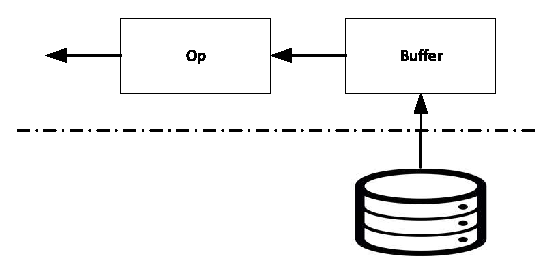
\includegraphics[width=0.5\linewidth]{handout/img/5-sigma.eps}
    \caption{选择算子实现}\label{fig:5-sigma}
\end{figure}

在bag模型或者set模型上做选择$\sigma$，输出都是bag模型，并且是tuple级别流式输出。下一章将会了解到$\sigma$下推是一个比较常用的逻辑优化方案。

\subsection*{$\pi_L(R)$}

在关系$R$上做投影$\pi_L(R)$，只需要逐个调入所有page，然后纵向截取tuple的属性即可，如\figurename\ref{fig:5-sigma}。由于需要调入所有page，它的性能是$B(R)$，内存约束是$1$。

SQL中支持扩展投影，所谓扩展投影是指$L$不仅仅是属性列表，还可以是一个判断表达式。是否是扩展投影，对方案没有影响，都必须调入所有page然后裁剪。

在set模型上做投影$\pi$，如果$L$包含主键，输出是set模型。算法支持tuple级别流式输出。$\pi$下推是一个比较常用的逻辑优化方案。

\subsection*{$\delta(R)$}

对于表空间存储的表来说，是不会有重复项的，重复项一般出现在中间结果中。去重算子$\delta(R)$挨个枚举所有page，如\figurename\ref{fig:5-delta}，同时建立一个内存索引，如果在索引中找到一条记录，则丢弃。由于需要调入所有page，它的性能是$B(R)$，不考虑索引开销的情况下内存约束是$1$。

\begin{figure}[H]
    \centering
    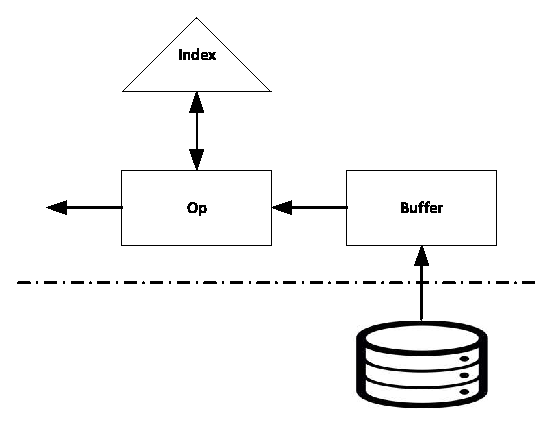
\includegraphics[width=0.5\linewidth]{handout/img/5-delta.eps}
    \caption{去重算子实现}\label{fig:5-delta}
\end{figure}

消除副本的一种开销最小的方案是采用bloom filter高概率的确定没有tuple存在。最后，去重算子支持流式输出。

\subsection*{$\tau(R)$}

单轮算法的排序方案，如\figurename\ref{fig:5-tau}，利用中间缓冲保存结果，在排完序后输出。如果中间缓冲能够兜住关系$R$，$\tau$的性能是$B(R)$，内存约束是$B(R)$。

\begin{figure}[H]
    \centering
    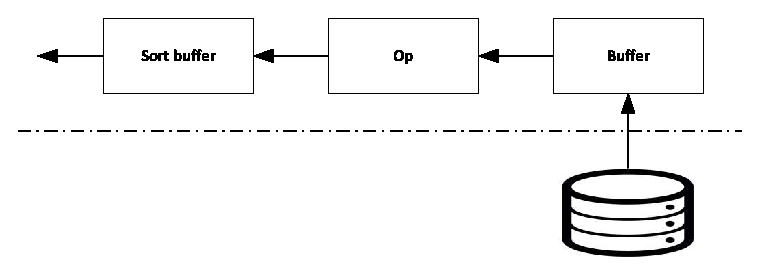
\includegraphics[width=0.8\linewidth]{handout/img/5-tau.eps}
    \caption{排序算子实现}\label{fig:5-tau}
\end{figure}

排序算子$\tau(R)$在完成前，无法输出。在后文的多路归并中，如果先保证部分有序，可以支持tuple级别流式输出。

在实现中，由于排序一般直接使用quick sort，要求连续大块内存。\figurename\ref{fig:5-tau}中的排序缓冲需要单独配置，PostgreSQL/Innodb中缺省在4MB左右。可以考虑使用内存版本的btree，这样可以直接使用buffer管理器的分页内存。此时，调入buffer的page不能swap到硬盘，同时在buffer中构建一个内存版本btree作为索引，当该表的所有页面调入完毕，内存btree索引构建完成，按照索引输出，结构上参考\figurename\ref{fig:5-delta}。

\subsection*{$\gamma_L(R)$}

在SQL语言中，GROUP BY将表中的tuple按照属性分成多个组，这些分组可以利用聚合函数做进一步处理，不加聚合函数的分组输出类似于排序$\tau(R)$，它的处理方案如\figurename\ref{fig:5-tau}。先按照分组构建一个索引，这个索引可能是键重复的，然后读入所有page，枚举tuple。当枚举完所有tuple，按照索引输出。

\begin{lstlisting}[style=verbose]
SELECT name, gender FROM employee GROUP BY gender, name
\end{lstlisting}

加了聚合函数处理的分组查询，由于输出的聚合结果，不需要保留分组后的表。由于聚合的结果一般是一个标量，所以输出的结果尺寸比较小，内存约束大致等于一个索引的大小。

下面这条语句对先按照column\_name属性分组，然后做聚合操作，最终的计算结果是一张表，表以column\_name为键，另一个属性是聚合函数计算出来的标量。

\begin{lstlisting}[style=verbose]
SELECT column_name, aggregate_function(column_name)
FROM table_name
WHERE column_name operator value
GROUP BY column_name
\end{lstlisting}

如果存在索引，并且按照索引分组做聚合，则可以利用索引直接处理，不需要调入page，性能很高。

与排序$\tau$类似，分组$\gamma$必须等待所有结果处理完毕后，才能输出。

\subsection*{$R \cup S$}

两个bag模型关系的并$R \cup S$，只需将两个关系合并即可。逻辑上需要枚举两个关系的所有page，但实际上可以做一个简单的记号即可。

\subsection*{$R \cap S$}

两个bag模型关系的交$R \cap S$，先将关系$R$逐page调入内存，建立$R$的索引并记录相同tuple出现的次数，然后丢弃掉该page。再将关系$S$逐page调入内存，比较tuple，如果一个tuple在索引中出现，则将引用计数减1，然后输出；否则丢弃。它的性能是$B(R)+B(S)$，内存约束是$1$。

\begin{figure}[H]
    \centering
    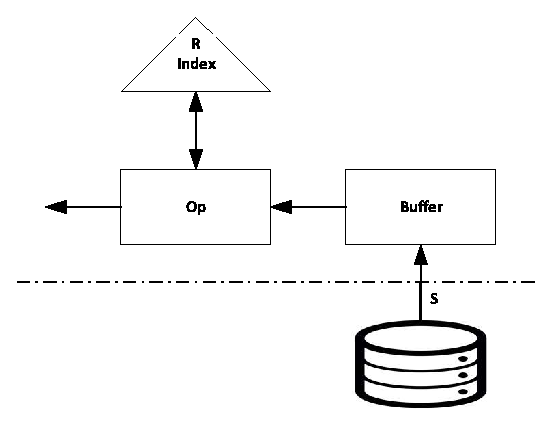
\includegraphics[width=0.6\linewidth]{handout/img/5-cap.eps}
    \caption{交算子实现}\label{fig:5-cap}
\end{figure}

以上是bag模型实现，但考虑到引入bag模型无非是为了方便实现，其实基于bag模型的交实现比set交要复杂一些。bag交与set交的实现，仅在$R$全部调入内存后，支持tuple级别流式操作。

\begin{exercise}
    设计set交方案。
\end{exercise}

\subsection*{$R - S$}

两个bag模型关系的差$R - S$，如\figurename\ref{fig:5-minus}，先将关系$R$逐page调入内存，然后建立索引记录次数，再将关系$S$逐page调入内存，比较tuple，当引用计数减到0，删除索引条目；如果$S$的tuple没有命中索引条目，直接drop掉。当$S$的所有tuple枚举完毕，按照索引输出。它的性能是$B(R)+B(S)$，内存约束是$B(R)+1$。如果存在索引，就更简单一些。

\begin{figure}[H]
    \centering
    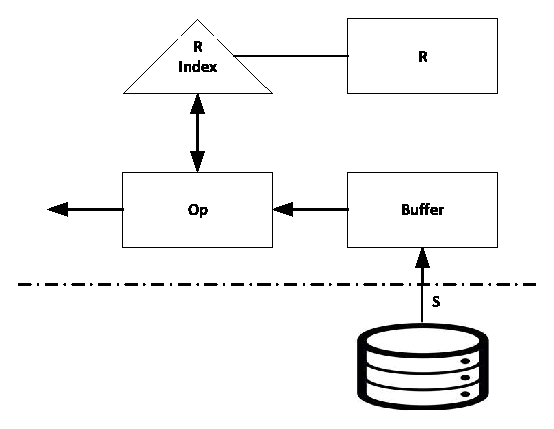
\includegraphics[width=0.6\linewidth]{handout/img/5-minus.eps}
    \caption{差算子实现}\label{fig:5-minus}
\end{figure}

差算子必须等结果计算完毕后才能输出。

\begin{exercise}
    设计set差方案。
\end{exercise}

\subsection*{$R \times S$}

两个bag模型关系的积$R \times S$，需要将$R$中的tuple与$S$中的每个tuple做合并处理，先将$S$整体调入内存，然后再逐个调入$R$的page，结构如\figurename\ref{fig:5-minus}。如果$min(B(R),B(S))+1 \le M$，性能是$B(R)+B(S)$，内存约束是$min(B(R),B(S))+1$。乘积可以直接tuple输出。

\subsection*{$R \bowtie S$}

两个bag模型关系的积$R \bowtie S$，需要将$R$和$S$中的tuple按照某个属性做连接处理。先将$S$整体调入内存，然后再逐个调入$R$的page，结构如\figurename\ref{fig:5-minus}。$min(B(R),B(S))+1 \le M$，性能是$B(R)+B(S)$，内存约束是$min(B(R),B(S))+1$。连接可以直接tuple输出。

总结一下，单目、双目算子在单轮算法的性能如\tablename\ref{tab:5-single}。
\begin{table}[H]
    \centering
    \caption{单轮算法性能表}\label{tab:5-single}
    \begin{tabular}{lccc}
        \toprule
        算子 & 内存约束 & 磁盘IO & 流输出 \\
        \midrule
        $\sigma, \pi, \delta$ & $1$ & $B$ & \checkmark \\
        $\gamma, \tau$        & $B < M$ & $B$ & \ding{55} \\
        $\cup$                & $1$ & $B(R) + B(S)$ & \checkmark \\
        $\cap$                & $1$ & $B(R) + B(S)$ & \checkmark \\
        $-$                   & $B(R) < M$ & $B(R) + B(S)$ & \ding{55} \\
        $\times, \bowtie, \bowtie_C$ & $min(B(R),B(S))) < M$ & $B(R) + B(S)$ & \checkmark \\
        \bottomrule
    \end{tabular}
\end{table}

在\tablename\ref{tab:5-single}中，$\sigma, \pi, \delta, \cup$这几个算子的内存约束仅为1，又支持流输出，后续将不再关注这几个算子的实现，这些算子均采用单轮算法。后面主要关注$\gamma, \tau, -, \times, \bowtie, \bowtie_C$这几个算子。

\section{nested-loop}

嵌套循环主要用于实现$\times, \bowtie, \bowtie_C$这几个算子。

\subsection*{$R \times S$}

假设$min(B(R),B(S)) > M$，无法使用单轮算法。嵌套循环比较直观，尽可能的调入$R$或$S$，设调入部分是$S_1$，然后逐page调入$R$，将$R$的tuple与$S_1$的tuple组合；然后再尽可能调入$S_2$，重复上述动作。

\begin{figure}[H]
    \centering
    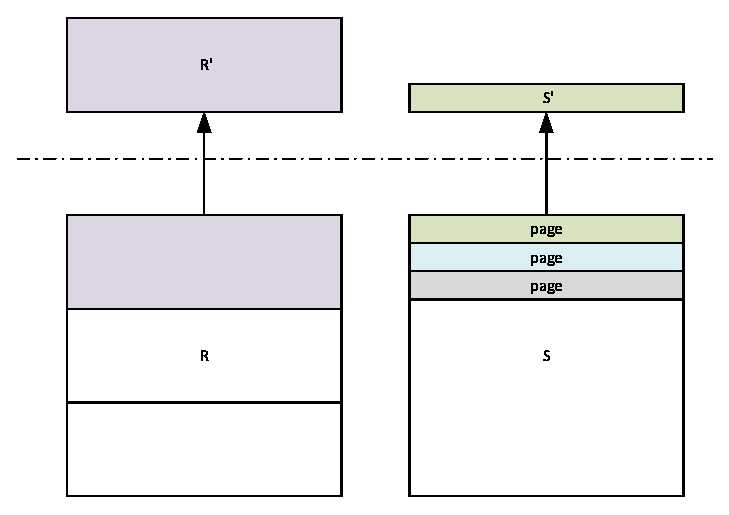
\includegraphics[width=0.8\linewidth]{handout/img/5-nested.eps}
    \caption{积算子nested-loop实现}\label{fig:5-nested}
\end{figure}

如\figurename\ref{fig:5-nested}所示，nested-loop算法先尽可能将$R$调入内存，然后逐个将$S$的页面调入内存，与$R$的每个tuple组合。

在\figurename\ref{fig:5-nested}中，$R$会调入一轮，$S$会调入$B(S)B(R)/M$轮，支持tuple流输出。对于$\times$算子，nested-loop是一个重要实现，后面介绍的排序归并方案中，排序无助于提升性能。

\subsection*{$R \bowtie S$}

方案与$R \times S$相同。

\section{两轮算法}

单轮算法要求关系能被整体调入内存，如果关系的尺寸很大，难以做到。两轮、多轮算法首先将关系排序，持久化后再做进一步处理，内存约束可以小于$M$，多路归并是一类通用的算子实现方案。在分布式系统中，多路归并与mapreduce、spark这样的任务调度框架相结合，用途很广。

\subsection*{$\tau$}

根据\tablename\ref{tab:5-single}，$B > M$无法使用单轮算法。两轮多路归并排序算法$\tau$如图\ref{fig:5-sort}所示，算法分为两个轮：
\begin{enumerate}
    \item 将$R$均分为$M$个分片，每个分片大小为$B(R)/M$。每次读入一个分片，然后排序，将排序后分片写入磁盘；
    \item 从$M$个分片读1个page，在每个分片上设置一个指针。分片已经排序，指针按照顺序枚举所有记录。merge算子从$M$个指针指向的记录中选取最小的记录输出。
\end{enumerate}

\begin{figure}[H]
    \centering
    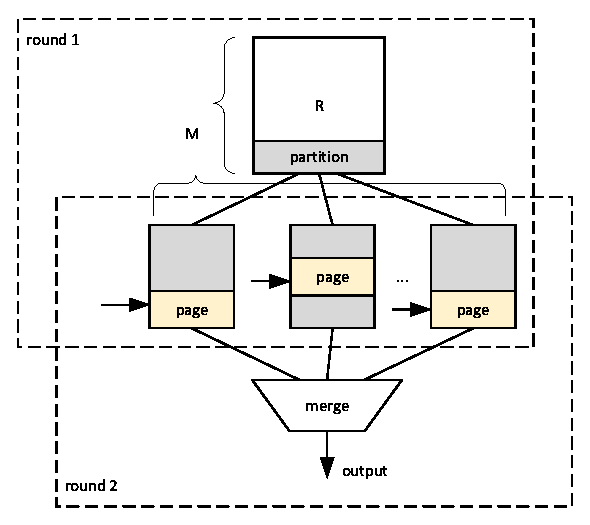
\includegraphics[width=0.8\linewidth]{handout/img/5-sort.eps}
    \caption{排序归并算法$\tau$实现}\label{fig:5-sort}
\end{figure}

两轮多路归并排序，在第2轮，不考虑输出buffer，至多能容纳$M$个块，内存约束是$M < B(R) < M*M$。一般情况下，两轮多路归并排序可以处理大多数关系，但是有些表尺寸太大，会超过这个内存约束，此时会用到某个的多轮多路归并算法处理。

两轮多路归并排序在第1轮读入$B$个块，写出$B$个块，第2轮读入$B$个块，所以磁盘IO开销是$3B$。得益于分片是排序的，方案在第2轮支持tuple流输出。

\subsection*{$\gamma$}

分组后如果使用聚合函数，在第2轮归并后应用聚合函数。

\begin{exercise}
    设计$\gamma$算子的两轮多轮归并算法。
\end{exercise}

\subsection*{$-$}

差算子在$B(R) < M$时，无法使用单轮算法。两轮多路归并的差算子实现如\figurename\ref{fig:5-minus2}所示，先将$R, S$分为$M$个分片，每个分片大小为$(B(R)+B(S))/M$，对每个分片排序后回写到硬盘。在第2轮，调入$R,S$的$M$个分片，从$R, S$的分片中选取最小的记录。bag模型下，如果两条记录匹配，则drop掉，否则输出$R$的最小记录。

\begin{figure}[H]
    \centering
    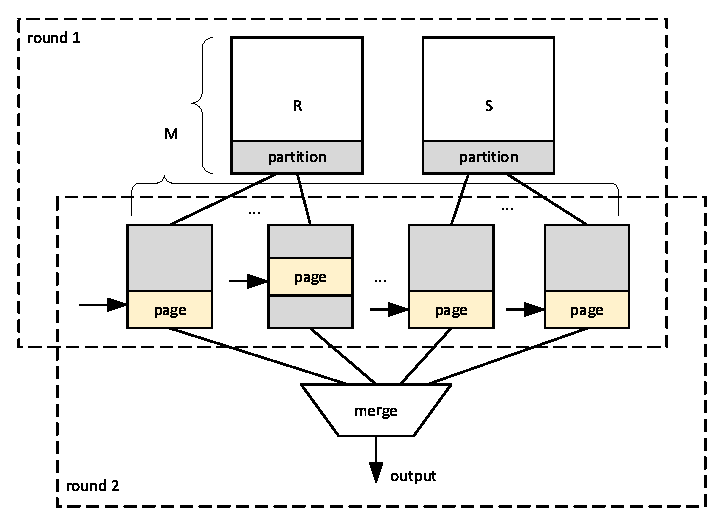
\includegraphics[width=\linewidth]{handout/img/5-minus2.eps}
    \caption{差算子两轮多路归并实现}\label{fig:5-minus2}
\end{figure}

\figurename\ref{fig:5-minus2}的方案中，$R,S$被调入两轮，开销是$3(B(R) + B(S))$。在第2轮开始后，支持tuple流输出，内存约束是$(B(R)+B(S) )< M^2$。

两轮多路归并差算子的方案可以进一步优化，先调入$S$，同时构造一个索引。然后对$R$做多路归并，每次从$R$的分片中选取最小的记录，与索引中的记录匹配。如果匹配，则drop掉，否则输出$R$的最小记录。

\begin{figure}[H]
    \centering
    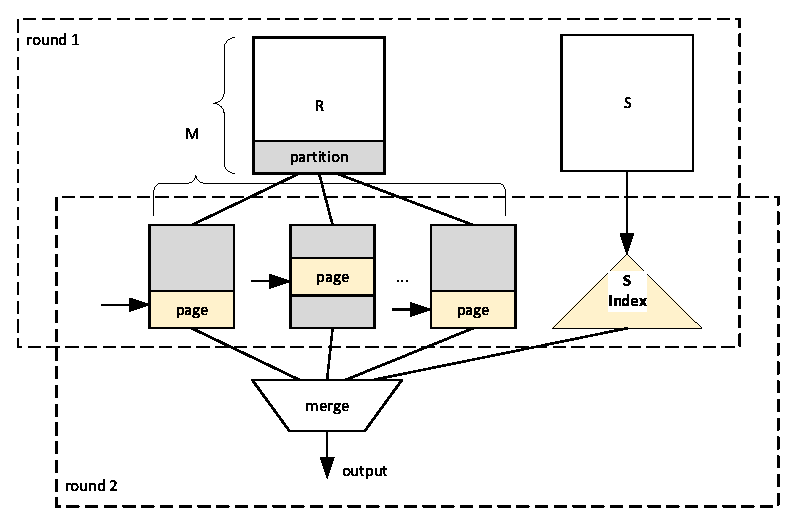
\includegraphics[width=\linewidth]{handout/img/5-minus3.eps}
    \caption{差算子两轮多路归并优化实现}\label{fig:5-minus3}
\end{figure}

\figurename\ref{fig:5-minus3}的方案中，$R$被调入两轮，$S$被调入一轮，开销是$3B(R) + B(S)$。在第2轮开始后，支持tuple流输出，内存约束是$B(R) < M^2$。

\begin{exercise}
    在\figurename\ref{fig:5-minus3}方案下，讨论bag和set模型的实现差异。
\end{exercise}

\subsection*{$\bowtie$}

\subsubsection*{基本方案}

$\bowtie$基本方案如\figurename\ref{fig:5-minus2}所示，先将$R, S$分为$M$个分片，每个分片大小为$(B(R)+B(S))/M$，对每个分片排序后回写到硬盘。在第2轮，调入$R,S$的$M$个分片，从$R, S$的分片中选取最小的记录。如果两条记录匹配，则输出，否则drop掉。

这个方案有一个潜在的问题：假设$S$的一条记录与$R$分片中的记录可以连接，然后移动$R$分片上的指针，当指针耗尽了分片上该page的所有记录，就应该调入下一个页面。此时，假设$S$的另一个分片上的记录也可以连接，但这个分片上的记录已经错失了机会。

这个问题在bag模型下尤为突出，set模型会好些，但仍然会出问题，问题的本质是$R,S$可连接的记录延展到多个page，如\figurename\ref{fig:5-join}所示。

\begin{figure}[H]
    \centering
    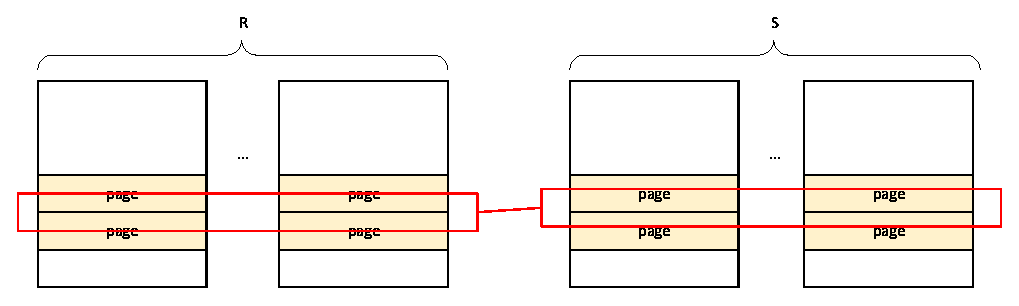
\includegraphics[width=\linewidth]{handout/img/5-join.eps}
    \caption{连接算子的潜在问题}\label{fig:5-join}
\end{figure}

\subsubsection*{改进方案}

一个改进方案是三轮，如\figurename\ref{fig:5-join2}所示。
\begin{enumerate}
    \item 用两轮多路归并方案分别对$R,S$排序，排序后回写磁盘。
    \item 采用两路归并处理$R\bowtie S$，这样就尽可能的在$M$内存大小容纳$R,S$的可连接记录。
\end{enumerate}

\begin{figure}[H]
    \centering
    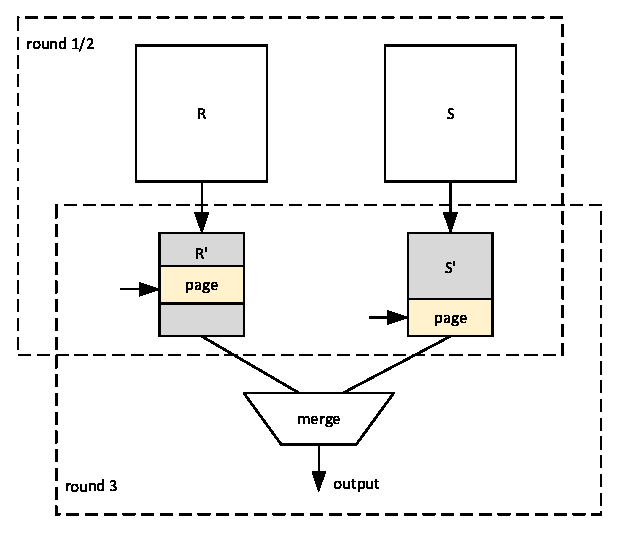
\includegraphics[width=0.8\linewidth]{handout/img/5-join2.eps}
    \caption{连接算子改进方案}\label{fig:5-join2}
\end{figure}

这个改进方案跑了三轮，io开销是$3(B(R) + B(S))$，并且仍然不能完全杜绝连接算子的潜在问题。

\subsubsection*{进一步改进}

对$R\bowtie S$的进一步改进，如\figurename\ref{fig:5-join3}所示。
\begin{enumerate}
    \item 对$R,S$分片，分片大小为$(B(R)+B(S))/M$。将分片调入内存，对$R,S$分别构建索引，索引指向排序后的分片。
    \item 按照$R,S$的索引，做zig-zag扫描，进行匹配，匹配成功调入$R,S$排序好的分片，进行连接。
    \item 如果$R,S$的可连接记录数在$M$内存中兜不住，产生内存溢出则使用前述的nested-loop方案处理。
\end{enumerate}

\begin{figure}[H]
    \centering
    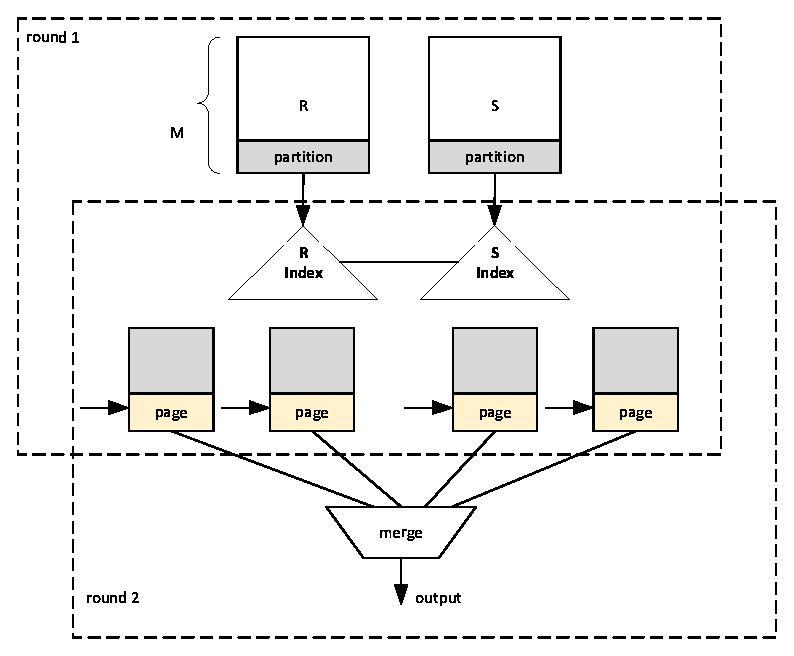
\includegraphics[width=\linewidth]{handout/img/5-join3.eps}
    \caption{连接算子进一步改进}\label{fig:5-join3}
\end{figure}

\figurename\ref{fig:5-join3}的性能基本是$3(B(R) + B(S))$，内存约束是$(B(R)+B(S) )< M^2$，在第2轮可以tuple流输出。

总结一下两类多路归并算法，如\tablename\ref{tab:5-two}所示。

\begin{table}[H]
    \centering
    \caption{两轮算法性能表}\label{tab:5-two}
    \begin{tabular}{lccc}
        \toprule
        算子 & 内存约束 & 磁盘IO & 流输出 \\
        \midrule
        $\tau, \gamma$ & $M < B(R) < M^2$ & $3B$ & \checkmark \\
        $-$   & $M < B(R) < M^2$ & $3B(R) + B(S)$ & \checkmark \\
        $\bowtie$ & $M < (B(R) + B(S)) < M^2$ & $3(B(R) + B(S))$ & \checkmark \\
    \bottomrule
    \end{tabular}
\end{table}

\subsection{多轮算法}

递归的多轮排序$\tau$算法如下：

\textbf{基础}：如果$R$能够整体调入$M$，采用单轮排序算法处理$R$，然后写盘。

\textbf{递推}：如果$R$不能整体调入$M$，将$R$拆分成$M$个子表$R_1, R_2, ..., R_M$。然后递归地对每个$R_i$做排序，最后对$M$个子表做多路归并。

其余多轮算法可以模仿这个排序算法处理，这个多轮算法将单轮、双轮、多轮集成到一个框架，简化了算法选择。

\section{基于索引的算法}

索引相较于数据，尺寸要小得多，可以利用索引来快速定位需要加载的page。采用索引来实现算法的问题是，当沿着索引扫描，可能会遇到一个page被反复加载的问题。没法完全规避这个问题，但是考虑到缓冲层的存在，page被反复加载的概率比较小。

在前述递归多路归并基础上，如果表上有索引，要优先采用索引来处理。现在重新考虑如下算子的实现方案：$\sigma, \delta, \tau, \gamma, \cap, -, \bowtie$。

\subsection*{$\sigma$}

在索引上根据$\sigma_{a=v}(R)$查找，根据条目调入相应的page。如果索引是聚集的，平均指标为$B(R)/V(R,a)$，其中$V(R,a)$是$R.a$不同属性数量，实际的指标可能要比这个值高一些。

如果索引是非聚集的，索引的tuple散布在各个page上，并且$R.a=v$条件可能会对应于多个tuple，$T(R)/V(R,a)$是这个条件平均需要访问的page数目，性能大约是$min(B(R), T(R)/V(R,a))$。

举例而言，假设$B(R)=1000$，$T(R)=20000$，即$R$有20000个tuple存放在1000个page上。考虑$R$的$a$属性上的$\sigma_{a=v}(R)$操作：
\begin{enumerate}
    \item 如果$R$聚集，不使用索引，磁盘IO为$B(R)$
    \item 如果$R$非聚集，不使用索引，磁盘IO为$T(R)$
    \item 假设$V(R,a)=100$，聚集索引，$\sigma_{a=v}(R)$操作的平均磁盘IO为$B(R)/V(R,a)=10$，再加上索引的IO数量
    \item 假设$V(R,a)=10$，非聚集索引，$\sigma_{a=v}(R)$操作的平均磁盘IO为$T(R)/V(R,a)=2000$，再加上索引的IO数量
    \item 假设$V(R,a)=20000$，$a$是$R$的主键，$\sigma_{a=v}(R)$操作的平均磁盘IO为1，再加上索引的IO数量
\end{enumerate}

上述的选择是一种简单的相等$\sigma_{a=v}(R)$操作，如果查询的条件更复杂，比如$\sigma_{a \ge 10\ \sf{AND}\ a \le 20}(R)$，可以在btree上处理。同时，对形如$\sigma_{a=v\ \sf{AND}\ C'}(R)$这样的复杂查询，可以先花少量磁盘IO处理$R.a=v$，然后再处理$C'$条件。

\subsection*{$\bowtie$}

两个表做自然连接$R(X,Y) \bowtie S(Y,Z)$，如果$R,S$上都有索引，可以采用\figurename\ref{fig:5-zigzag}的zig-zag扫描方案。沿着索引$R.Y$和$S.Y$移动指针，找到匹配的tuple，做自然连接。整个动作过程就象啮合的两个齿轮，称为zig-zag扫描。

\begin{figure}[H]
    \centering
    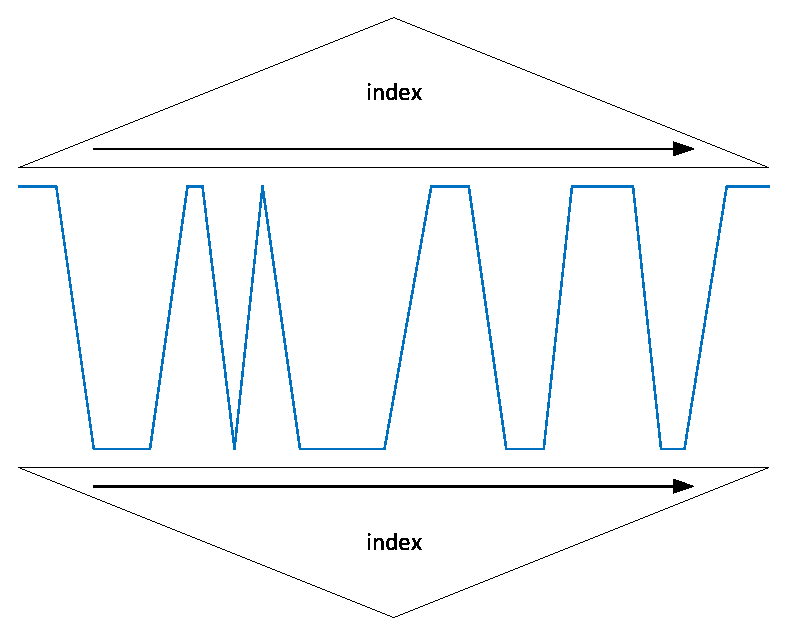
\includegraphics[width=0.5\linewidth]{handout/img/5-zigzag.eps}
    \caption{zig-zag扫描}\label{fig:5-zigzag}
\end{figure}

如果$R$是聚集的，枚举$R$需要$B(R)$的磁盘IO；如果如果$R$是非聚集的，枚举$R$需要$T(R)$的磁盘IO。

每个$R$的tuple平均需要读取$T(S)/V(S,Y)$个$S$上的tuple。如果$Y$是$S$的非聚集索引，则平均磁盘IO开销为$T(S)/V(S,Y)$。如果$Y$是$S$的聚集索引，平均磁盘IO开销为$max(1,B(S)/V(S,Y))$。


\section{算子连接}

SQL语句被解析成算子表达式，经过优化后要得到一个执行计划，执行计划中各个算子的实现算法需要彼此连接起来，关系和中间计算结果要流经各个算法，最终得到SQL查询结果。

本节讨论如何将各个算子连接起来，数据如何流经各个算子。一般来说，算子的组合主要有两种方式：一是tuple流，二是\emph{物化}，所谓物化是指中间计算结果以关系的形式被完整保存在磁盘上。在分布式系统中，算子连接还涉及mapreduce、spark这样的调度框架。

\begin{figure}[H]
    \centering
    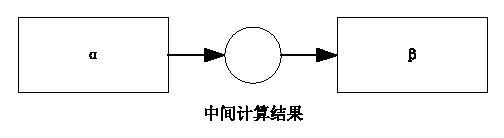
\includegraphics[width=0.7\linewidth]{handout/img/5-connect.eps}
    \caption{两个算子连接}\label{fig:5-connect}
\end{figure}

用函数的形式表示算子，假设两个算子$\alpha, \beta$，在算子表达式表示为$\alpha\beta(R)$。如果$\beta(R)$输出tuple流，并且$\alpha$接受tuple流，就可以将两个算法用tuple串联起来。

\subsection{迭代器}

关系算子的实现往往依赖于一个更基础的算子——迭代。迭代器可以看成一个对象，它暴露一个next()函数，该函数返回一条记录。基础的迭代器包括：
\begin{itemize}
    \item tablescan，按照page迭代
    \item indexscan，按照索引迭代
    \item pagescan，枚举一个page内部的tuple
\end{itemize}
